% Options for packages loaded elsewhere
\PassOptionsToPackage{unicode}{hyperref}
\PassOptionsToPackage{hyphens}{url}
%
\documentclass[
  ignorenonframetext,
  aspectratio=169,
]{beamer}
\usepackage{pgfpages}
\setbeamertemplate{caption}[numbered]
\setbeamertemplate{caption label separator}{: }
\setbeamercolor{caption name}{fg=normal text.fg}
\beamertemplatenavigationsymbolsempty
% Prevent slide breaks in the middle of a paragraph
\widowpenalties 1 10000
\raggedbottom
\setbeamertemplate{part page}{
  \centering
  \begin{beamercolorbox}[sep=16pt,center]{part title}
    \usebeamerfont{part title}\insertpart\par
  \end{beamercolorbox}
}
\setbeamertemplate{section page}{
  \centering
  \begin{beamercolorbox}[sep=12pt,center]{part title}
    \usebeamerfont{section title}\insertsection\par
  \end{beamercolorbox}
}
\setbeamertemplate{subsection page}{
  \centering
  \begin{beamercolorbox}[sep=8pt,center]{part title}
    \usebeamerfont{subsection title}\insertsubsection\par
  \end{beamercolorbox}
}
\AtBeginPart{
  \frame{\partpage}
}
\AtBeginSection{
  \ifbibliography
  \else
    \frame{\sectionpage}
  \fi
}
\AtBeginSubsection{
  \frame{\subsectionpage}
}

\usepackage{amsmath,amssymb}
\usepackage{lmodern}
\usepackage{iftex}
\ifPDFTeX
  \usepackage[T1]{fontenc}
  \usepackage[utf8]{inputenc}
  \usepackage{textcomp} % provide euro and other symbols
\else % if luatex or xetex
  \usepackage{unicode-math}
  \defaultfontfeatures{Scale=MatchLowercase}
  \defaultfontfeatures[\rmfamily]{Ligatures=TeX,Scale=1}
\fi
% Use upquote if available, for straight quotes in verbatim environments
\IfFileExists{upquote.sty}{\usepackage{upquote}}{}
\IfFileExists{microtype.sty}{% use microtype if available
  \usepackage[]{microtype}
  \UseMicrotypeSet[protrusion]{basicmath} % disable protrusion for tt fonts
}{}
\makeatletter
\@ifundefined{KOMAClassName}{% if non-KOMA class
  \IfFileExists{parskip.sty}{%
    \usepackage{parskip}
  }{% else
    \setlength{\parindent}{0pt}
    \setlength{\parskip}{6pt plus 2pt minus 1pt}}
}{% if KOMA class
  \KOMAoptions{parskip=half}}
\makeatother
\usepackage{xcolor}
\newif\ifbibliography
\setlength{\emergencystretch}{3em} % prevent overfull lines
\setcounter{secnumdepth}{-\maxdimen} % remove section numbering

\usepackage{color}
\usepackage{fancyvrb}
\newcommand{\VerbBar}{|}
\newcommand{\VERB}{\Verb[commandchars=\\\{\}]}
\DefineVerbatimEnvironment{Highlighting}{Verbatim}{commandchars=\\\{\}}
% Add ',fontsize=\small' for more characters per line
\usepackage{framed}
\definecolor{shadecolor}{RGB}{241,243,245}
\newenvironment{Shaded}{\begin{snugshade}}{\end{snugshade}}
\newcommand{\AlertTok}[1]{\textcolor[rgb]{0.68,0.00,0.00}{#1}}
\newcommand{\AnnotationTok}[1]{\textcolor[rgb]{0.37,0.37,0.37}{#1}}
\newcommand{\AttributeTok}[1]{\textcolor[rgb]{0.40,0.45,0.13}{#1}}
\newcommand{\BaseNTok}[1]{\textcolor[rgb]{0.68,0.00,0.00}{#1}}
\newcommand{\BuiltInTok}[1]{\textcolor[rgb]{0.00,0.23,0.31}{#1}}
\newcommand{\CharTok}[1]{\textcolor[rgb]{0.13,0.47,0.30}{#1}}
\newcommand{\CommentTok}[1]{\textcolor[rgb]{0.37,0.37,0.37}{#1}}
\newcommand{\CommentVarTok}[1]{\textcolor[rgb]{0.37,0.37,0.37}{\textit{#1}}}
\newcommand{\ConstantTok}[1]{\textcolor[rgb]{0.56,0.35,0.01}{#1}}
\newcommand{\ControlFlowTok}[1]{\textcolor[rgb]{0.00,0.23,0.31}{#1}}
\newcommand{\DataTypeTok}[1]{\textcolor[rgb]{0.68,0.00,0.00}{#1}}
\newcommand{\DecValTok}[1]{\textcolor[rgb]{0.68,0.00,0.00}{#1}}
\newcommand{\DocumentationTok}[1]{\textcolor[rgb]{0.37,0.37,0.37}{\textit{#1}}}
\newcommand{\ErrorTok}[1]{\textcolor[rgb]{0.68,0.00,0.00}{#1}}
\newcommand{\ExtensionTok}[1]{\textcolor[rgb]{0.00,0.23,0.31}{#1}}
\newcommand{\FloatTok}[1]{\textcolor[rgb]{0.68,0.00,0.00}{#1}}
\newcommand{\FunctionTok}[1]{\textcolor[rgb]{0.28,0.35,0.67}{#1}}
\newcommand{\ImportTok}[1]{\textcolor[rgb]{0.00,0.46,0.62}{#1}}
\newcommand{\InformationTok}[1]{\textcolor[rgb]{0.37,0.37,0.37}{#1}}
\newcommand{\KeywordTok}[1]{\textcolor[rgb]{0.00,0.23,0.31}{#1}}
\newcommand{\NormalTok}[1]{\textcolor[rgb]{0.00,0.23,0.31}{#1}}
\newcommand{\OperatorTok}[1]{\textcolor[rgb]{0.37,0.37,0.37}{#1}}
\newcommand{\OtherTok}[1]{\textcolor[rgb]{0.00,0.23,0.31}{#1}}
\newcommand{\PreprocessorTok}[1]{\textcolor[rgb]{0.68,0.00,0.00}{#1}}
\newcommand{\RegionMarkerTok}[1]{\textcolor[rgb]{0.00,0.23,0.31}{#1}}
\newcommand{\SpecialCharTok}[1]{\textcolor[rgb]{0.37,0.37,0.37}{#1}}
\newcommand{\SpecialStringTok}[1]{\textcolor[rgb]{0.13,0.47,0.30}{#1}}
\newcommand{\StringTok}[1]{\textcolor[rgb]{0.13,0.47,0.30}{#1}}
\newcommand{\VariableTok}[1]{\textcolor[rgb]{0.07,0.07,0.07}{#1}}
\newcommand{\VerbatimStringTok}[1]{\textcolor[rgb]{0.13,0.47,0.30}{#1}}
\newcommand{\WarningTok}[1]{\textcolor[rgb]{0.37,0.37,0.37}{\textit{#1}}}

\providecommand{\tightlist}{%
  \setlength{\itemsep}{0pt}\setlength{\parskip}{0pt}}\usepackage{longtable,booktabs,array}
\usepackage{calc} % for calculating minipage widths
\usepackage{caption}
% Make caption package work with longtable
\makeatletter
\def\fnum@table{\tablename~\thetable}
\makeatother
\usepackage{graphicx}
\makeatletter
\def\maxwidth{\ifdim\Gin@nat@width>\linewidth\linewidth\else\Gin@nat@width\fi}
\def\maxheight{\ifdim\Gin@nat@height>\textheight\textheight\else\Gin@nat@height\fi}
\makeatother
% Scale images if necessary, so that they will not overflow the page
% margins by default, and it is still possible to overwrite the defaults
% using explicit options in \includegraphics[width, height, ...]{}
\setkeys{Gin}{width=\maxwidth,height=\maxheight,keepaspectratio}
% Set default figure placement to htbp
\makeatletter
\def\fps@figure{htbp}
\makeatother

\makeatletter
\makeatother
\makeatletter
\makeatother
\makeatletter
\@ifpackageloaded{caption}{}{\usepackage{caption}}
\AtBeginDocument{%
\ifdefined\contentsname
  \renewcommand*\contentsname{Table of contents}
\else
  \newcommand\contentsname{Table of contents}
\fi
\ifdefined\listfigurename
  \renewcommand*\listfigurename{List of Figures}
\else
  \newcommand\listfigurename{List of Figures}
\fi
\ifdefined\listtablename
  \renewcommand*\listtablename{List of Tables}
\else
  \newcommand\listtablename{List of Tables}
\fi
\ifdefined\figurename
  \renewcommand*\figurename{Figure}
\else
  \newcommand\figurename{Figure}
\fi
\ifdefined\tablename
  \renewcommand*\tablename{Table}
\else
  \newcommand\tablename{Table}
\fi
}
\@ifpackageloaded{float}{}{\usepackage{float}}
\floatstyle{ruled}
\@ifundefined{c@chapter}{\newfloat{codelisting}{h}{lop}}{\newfloat{codelisting}{h}{lop}[chapter]}
\floatname{codelisting}{Listing}
\newcommand*\listoflistings{\listof{codelisting}{List of Listings}}
\makeatother
\makeatletter
\@ifpackageloaded{caption}{}{\usepackage{caption}}
\@ifpackageloaded{subcaption}{}{\usepackage{subcaption}}
\makeatother
\makeatletter
\@ifpackageloaded{tcolorbox}{}{\usepackage[many]{tcolorbox}}
\makeatother
\makeatletter
\@ifundefined{shadecolor}{\definecolor{shadecolor}{rgb}{.97, .97, .97}}
\makeatother
\makeatletter
\makeatother
\ifLuaTeX
  \usepackage{selnolig}  % disable illegal ligatures
\fi
\IfFileExists{bookmark.sty}{\usepackage{bookmark}}{\usepackage{hyperref}}
\IfFileExists{xurl.sty}{\usepackage{xurl}}{} % add URL line breaks if available
\urlstyle{same} % disable monospaced font for URLs
\hypersetup{
  pdftitle={Multiple Regressions},
  pdfauthor={Year 2022-2023},
  hidelinks,
  pdfcreator={LaTeX via pandoc}}

\title{Multiple Regressions}
\subtitle{Data-Based Economics}
\author{Year 2022-2023}
\date{}

\begin{document}
\frame{\titlepage}
\ifdefined\Shaded\renewenvironment{Shaded}{\begin{tcolorbox}[frame hidden, interior hidden, boxrule=0pt, sharp corners, enhanced, breakable, borderline west={3pt}{0pt}{shadecolor}]}{\end{tcolorbox}}\fi

\begin{frame}{The problem}
\protect\hypertarget{the-problem}{}
\begin{block}{Remember dataset from last time}
\protect\hypertarget{remember-dataset-from-last-time}{}
\begin{columns}[T]
\begin{column}{0.48\textwidth}
\begin{longtable}[]{@{}lllll@{}}
\toprule()
& type & income & education & prestige \\
\midrule()
\endhead
accountant & prof & 62 & 86 & 82 \\
pilot & prof & 72 & 76 & 83 \\
architect & prof & 75 & 92 & 90 \\
author & prof & 55 & 90 & 76 \\
chemist & prof & 64 & 86 & 90 \\
\bottomrule()
\end{longtable}
\end{column}

\begin{column}{0.48\textwidth}
\begin{itemize}
\tightlist
\item
  Last week we ``ran'' a linear regression: \(y = \alpha + \beta x\).
  Result: \[\text{income} = xx + 0.72 \text{education}\]
\item
  Should we have looked at ``prestige'' instead ?
  \[\text{income} = xx + 0.83 \text{prestige}\]
\item
  Which one is better?
\end{itemize}
\end{column}
\end{columns}
\end{block}
\end{frame}

\begin{frame}[fragile]
\begin{block}{Prestige or Education}
\protect\hypertarget{prestige-or-education}{}
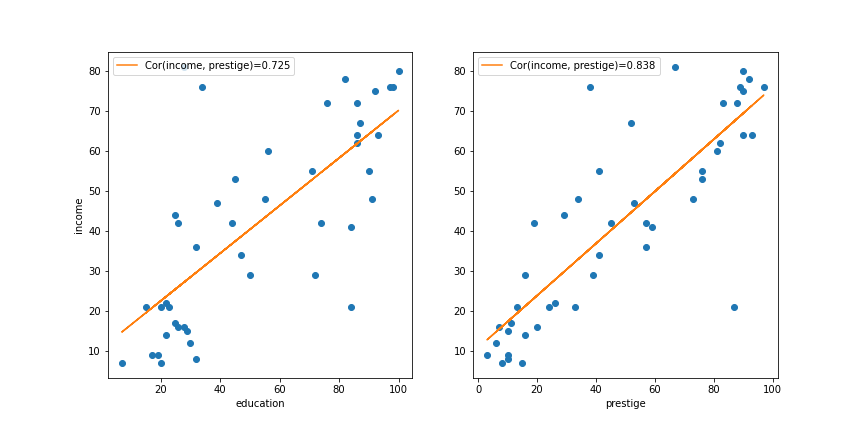
\includegraphics[width=0.8\textwidth,height=\textheight]{./graphs/prestige_or_education.png}

\begin{itemize}
\tightlist
\item
  if the goal is to predict: the one with higher explained variance

  \begin{itemize}
  \tightlist
  \item
    \texttt{prestige} has higher \(R^2\) (\(0.83^2\))
  \end{itemize}
\item
  unless we \emph{are} interested in the effect of education
\end{itemize}
\end{block}
\end{frame}

\begin{frame}
\begin{block}{Multiple regression}
\protect\hypertarget{multiple-regression}{}
\begin{itemize}
\tightlist
\item
  What about using both?

  \begin{itemize}
  \tightlist
  \item
    2 variables model:
    \[\text{income} = \alpha + \beta_1 \text{education} + \beta_2 \text{prestige}\]
  \item
    will \emph{probably} improve prediction power (explained variance)
  \item
    \(\beta_1\) might not be meaningful on its own anymore (education
    and prestige are correlated)
  \end{itemize}
\end{itemize}
\end{block}
\end{frame}

\begin{frame}
\begin{block}{Fitting a model}
\protect\hypertarget{fitting-a-model}{}
Now we are trying to fit a \textbf{plane} to a cloud of points.

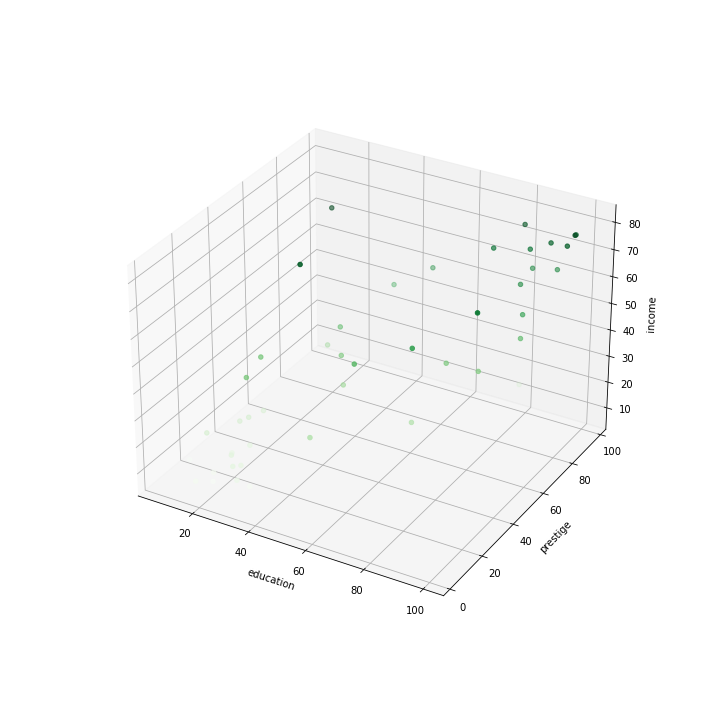
\includegraphics{graphs/empty_data.png}
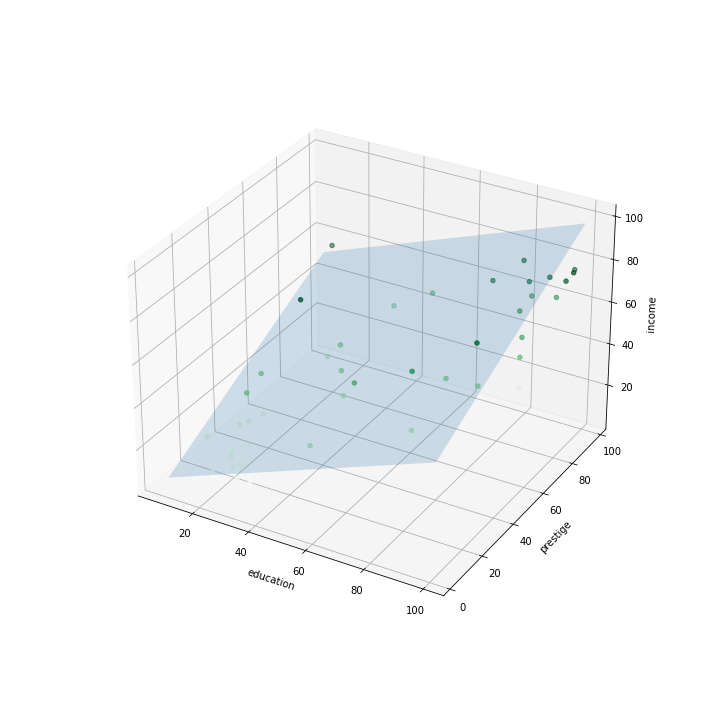
\includegraphics{graphs/2d_regression.png}
\end{block}
\end{frame}

\begin{frame}
\begin{block}{Minimization Criterium}
\protect\hypertarget{minimization-criterium}{}
\begin{itemize}
\tightlist
\item
  Take all observations:
  \((\text{income}\_n,\text{education}\_n,\text{prestige}\_n)\_{n\in[0,N]}\)
\item
  Objective: sum of squares
  \[ L(\alpha, \beta_1, \beta_2) = \sum_i \left( \underbrace{ \alpha + \beta_1 \text{education}\_n + \beta_2 \text{prestige}\_n - \text{income}\_n }\_{e_n=\text{prediction error} }\right)^2 \]
\item
  Minimize loss function in \(\alpha\), \(\beta_1\), \(\beta_2\)
\item
  Again, we can perform numerical optimization (machine learning
  approach)

  \begin{itemize}
  \tightlist
  \item
    \ldots{} but there is an explicit formula
  \end{itemize}
\end{itemize}
\end{block}
\end{frame}

\begin{frame}[fragile]
\begin{block}{Ordinary Least Square}
\protect\hypertarget{ordinary-least-square}{}
\begin{columns}[T]
\begin{column}{0.48\textwidth}
\[Y = \begin{bmatrix}
\text{income}_1 \\\\
\vdots \\\\
\text{income}_N 
\end{bmatrix}\] \[X = \begin{bmatrix}
1 & \text{education}_1 & \text{prestige}_1 \\\\
\vdots & \vdots & \vdots \\\\
1 &\text{education}_N & \text{prestige}_N
\end{bmatrix}\]
\end{column}

\begin{column}{0.48\textwidth}
\begin{itemize}
\tightlist
\item
  Matrix Version (look for
  \(B = \left( \alpha, \beta_1 , \beta_2 \right)\)): \[Y =  X B + E\]
\item
  Note that constant can be interpreted as a ``variable''
\item
  Loss function \[L(A,B) = (Y - X B)' (Y - X B)\]
\item
  Result of minimization \(\min_{(A,B)} L(A,B)\) :
  \[\begin{bmatrix}\alpha & \beta_1 & \beta_2 \end{bmatrix} = (X'X)^{-1} X' Y \]
\end{itemize}
\end{column}
\end{columns}
\end{block}

\begin{block}{Solution}
\protect\hypertarget{solution}{}
\begin{itemize}
\tightlist
\item
  Result:
  \[\text{income} = 10.43  + 0.03 \times \text{education} + 0.62 \times \text{prestige}\]
\item
  Questions:

  \begin{itemize}
  \tightlist
  \item
    is it a \emph{better} regression than the other?
  \item
    is the coefficient in front of \texttt{education} significant?
  \item
    how do we interpret it?
  \item
    can we build confidence intervals?
  \end{itemize}
\end{itemize}

\textless\textless\textless\textless\textless\textless\textless\textless{}
HEAD:session\_4/index.qmd \# Explained Variance ========
\end{block}
\end{frame}

\begin{frame}{Explained Variance}
\protect\hypertarget{explained-variance}{}
\end{frame}

\begin{frame}
\begin{quote}
\begin{quote}
\begin{quote}
\begin{quote}
\begin{quote}
\begin{quote}
\begin{quote}
\begin{quote}
f769a93bfa6a7cf861396754a3715ef9ed4a78a2:session\_4/index.md
\end{quote}
\end{quote}
\end{quote}
\end{quote}
\end{quote}
\end{quote}
\end{quote}
\end{quote}

\begin{block}{Explained Variance}
\protect\hypertarget{explained-variance-1}{}
\begin{itemize}
\tightlist
\item
  As in the 1d case we can compare:

  \begin{itemize}
  \tightlist
  \item
    the variability of the model predictions (\(MSS\))
  \item
    the variance of the data (\(TSS\), T for total)
  \end{itemize}
\item
  Coefficient of determination: \[R^2 = \frac{MSS}{TSS}\]
\item
  Or: \[R^2 = 1-\frac{RSS}{SST}\] where \(RSS\) is the non explained
  variance
\end{itemize}
\end{block}

\begin{block}{Adjusted R squared}
\protect\hypertarget{adjusted-r-squared}{}
\begin{columns}[T]
\begin{column}{0.48\textwidth}
\begin{itemize}
\tightlist
\item
  In our example:
\end{itemize}

\begin{longtable}[]{@{}
  >{\raggedright\arraybackslash}p{(\columnwidth - 4\tabcolsep) * \real{0.2151}}
  >{\raggedright\arraybackslash}p{(\columnwidth - 4\tabcolsep) * \real{0.0645}}
  >{\raggedright\arraybackslash}p{(\columnwidth - 4\tabcolsep) * \real{0.7204}}@{}}
\toprule()
\begin{minipage}[b]{\linewidth}\raggedright
Regression
\end{minipage} & \begin{minipage}[b]{\linewidth}\raggedright
\(R^2\)
\end{minipage} & \begin{minipage}[b]{\linewidth}\raggedright
{ \(R^2_{adj}\) }
\end{minipage} \\
\midrule()
\endhead
education & 0.525 & { 0.514 } \\
prestige & 0.702 & { 0.695 } \\
education + prestige & 0.7022 & { 0.688 } \\
\bottomrule()
\end{longtable}
\end{column}

\begin{column}{0.48\textwidth}
\begin{itemize}
\item
  Fact:

  \begin{itemize}
  \item
    adding more regressors always improve \(R^2\)
  \item
    why not throw everything in? (kitchen sink regressions)
  \item
    two many regressors: overfitting the data
  \end{itemize}
\item
  Penalise additional regressors: adjusted R\^{}2

  \begin{itemize}
  \tightlist
  \item
    example formula:

    \begin{itemize}
    \tightlist
    \item
      \(N\): number of observations
    \item
      \(p\) number of variables
      \[R^2_{adj} = 1-(1-R^2)\frac{N-1}{N-p-1}\]
    \end{itemize}
  \end{itemize}
\end{itemize}
\end{column}
\end{columns}
\end{block}
\end{frame}

\begin{frame}[fragile]{Interpretation and variable change}
\protect\hypertarget{interpretation-and-variable-change}{}
\begin{block}{Making a regression with statsmodels}
\protect\hypertarget{making-a-regression-with-statsmodels}{}
\begin{Shaded}
\begin{Highlighting}[]
\ImportTok{import}\NormalTok{ statsmodels}
\end{Highlighting}
\end{Shaded}

We use a special \texttt{API} inspired by \texttt{R}:

\begin{Shaded}
\begin{Highlighting}[]
\ImportTok{import}\NormalTok{ statsmodels.formula.api }\ImportTok{as}\NormalTok{ smf}
\end{Highlighting}
\end{Shaded}
\end{block}

\begin{block}{Performing a regression}
\protect\hypertarget{performing-a-regression}{}
\begin{itemize}
\tightlist
\item
  Running a regression with \texttt{statsmodels}
\end{itemize}

\begin{verbatim}
model = smf.ols('income ~ education',  df)  # model
res = model.fit()  # perform the regression
res.describe()
\end{verbatim}

\begin{itemize}
\tightlist
\item
  `income \textasciitilde{} education' is the model \emph{formula}
\end{itemize}

\begin{verbatim}
                            OLS Regression Results                            
==============================================================================
Dep. Variable:                 income   R-squared:                       0.525
Model:                            OLS   Adj. R-squared:                  0.514
Method:                 Least Squares   F-statistic:                     47.51
Date:                Tue, 02 Feb 2021   Prob (F-statistic):           1.84e-08
Time:                        05:21:25   Log-Likelihood:                -190.42
No. Observations:                  45   AIC:                             384.8
Df Residuals:                      43   BIC:                             388.5
Df Model:                           1                                         
Covariance Type:            nonrobust                                         
==============================================================================
                 coef    std err          t      P>|t|      [0.025      0.975]
==============================================================================
Intercept     10.6035      5.198      2.040      0.048       0.120      21.087
education      0.5949      0.086      6.893      0.000       0.421       0.769
==============================================================================
Omnibus:                        9.841   Durbin-Watson:                   1.736
Prob(Omnibus):                  0.007   Jarque-Bera (JB):               10.609
Skew:                           0.776   Prob(JB):                      0.00497
Kurtosis:                       4.802   Cond. No.                         123.
==============================================================================
\end{verbatim}
\end{block}

\begin{block}{Formula mini-language}
\protect\hypertarget{formula-mini-language}{}
\begin{itemize}
\tightlist
\item
  With \texttt{statsmodels} formulas, can be supplied with R-style
  syntax
\item
  Examples:
\end{itemize}

\begin{longtable}[]{@{}
  >{\raggedright\arraybackslash}p{(\columnwidth - 2\tabcolsep) * \real{0.3986}}
  >{\raggedright\arraybackslash}p{(\columnwidth - 2\tabcolsep) * \real{0.6014}}@{}}
\toprule()
\begin{minipage}[b]{\linewidth}\raggedright
Formula
\end{minipage} & \begin{minipage}[b]{\linewidth}\raggedright
Model
\end{minipage} \\
\midrule()
\endhead
\texttt{income\ \textasciitilde{}\ education} &
\(\text{income}_i = \alpha + \beta \text{education}_i\) \\
\texttt{income\ \textasciitilde{}\ prestige} &
\(\text{income}_i = \alpha + \beta \text{prestige}_i\) \\
\texttt{income\ \textasciitilde{}\ prestige\ -\ 1} &
\(\text{income}_i = \beta \text{prestige}_i\) (no intercept) \\
\texttt{income\ \textasciitilde{}\ education\ +\ prestige} &
\(\text{income}_i = \alpha + \beta_1 \text{education}_i + \beta_2 \text{prestige}_i\) \\
\bottomrule()
\end{longtable}
\end{block}

\begin{block}{Formula mini-language}
\protect\hypertarget{formula-mini-language-1}{}
\begin{itemize}
\tightlist
\item
  One can use formulas to apply transformations to variables
\end{itemize}

\begin{longtable}[]{@{}
  >{\raggedright\arraybackslash}p{(\columnwidth - 2\tabcolsep) * \real{0.3333}}
  >{\raggedright\arraybackslash}p{(\columnwidth - 2\tabcolsep) * \real{0.6667}}@{}}
\toprule()
\begin{minipage}[b]{\linewidth}\raggedright
Formula
\end{minipage} & \begin{minipage}[b]{\linewidth}\raggedright
Model
\end{minipage} \\
\midrule()
\endhead
\texttt{log(P)\ \textasciitilde{}\ log(M)\ +\ log(Y)} &
\(\log(P_i) = \alpha + \alpha_1 \log(M_i) + \alpha_2 \log(Y_i)\)
(log-log) \\
\texttt{log(Y)\ \textasciitilde{}\ i} & \(\log(P_i) = \alpha + i_i\)
(semi-logs) \\
\bottomrule()
\end{longtable}

\begin{itemize}
\tightlist
\item
  This is useful if the true relationship is nonlinear
\item
  Also useful, to interpret the coefficients
\end{itemize}
\end{block}

\begin{block}{Coefficients interpetation}
\protect\hypertarget{coefficients-interpetation}{}
\begin{itemize}
\tightlist
\item
  Example:

  \begin{itemize}
  \tightlist
  \item
    (\texttt{police\_spending} and \texttt{prevention\_policies} in
    million dollars)
    \[\text{number_or_crimes} = 0.005\% - 0.001 \text{pol_spend} - 0.005 \text{prev_pol} + 0.002 \text{population density}\]
  \end{itemize}
\item
  reads: \emph{when holding other variables constant a 0.1 million
  increase in police spending reduces crime rate by 0.001\%}
\item
  interpretation?

  \begin{itemize}
  \tightlist
  \item
    problematic because variables have different units
  \item
    we can say that prevention policies are more efficient than police
    spending \emph{ceteris paribus}
  \end{itemize}
\item
  Take logs:
  \[\log(\text{number_or_crimes}) = 0.005\% - 0.15 \log(\text{pol_spend}) - 0.4 \log(\text{prev_pol}) + 0.2 \log(\text{population density})\]

  \begin{itemize}
  \tightlist
  \item
    now we have an estimate of elasticities
  \item
    a \(1\%\) increase in police spending leads to a \(0.15\%\) decrease
    in the number of crimes
  \end{itemize}
\end{itemize}
\end{block}
\end{frame}

\begin{frame}{Statistical Inference}
\protect\hypertarget{statistical-inference}{}
\begin{block}{Hypotheses}
\protect\hypertarget{hypotheses}{}
\begin{columns}[T]
\begin{column}{0.48\textwidth}
\begin{itemize}
\item
  Recall what we do:

  \begin{itemize}
  \tightlist
  \item
    we have the data \(X,Y\)
  \item
    we choose a \emph{model}: \[ Y = \alpha + X \beta \]
  \item
    from the data we compute \emph{estimates}:
    \[\hat{\beta}  = (X'X)^{-1} X' Y \] \[\hat{\alpha} = Y- X \beta \]
  \item
    estimates are a precise function of data

    \begin{itemize}
    \tightlist
    \item
      exact formula not important here
    \end{itemize}
  \end{itemize}
\end{itemize}
\end{column}

\begin{column}{0.48\textwidth}
\begin{itemize}
\item
  We make some hypotheses on the data generation process:

  \begin{itemize}
  \tightlist
  \item
    \(Y = X \beta + \epsilon\)
  \item
    \(\mathbb{E}\left[ \epsilon \right] = 0\)
  \item
    \(\epsilon\) multivariate normal with covariance matrix
    \(\sigma^2 I_n\)

    \begin{itemize}
    \tightlist
    \item
      \(\forall i, \sigma(\epsilon_i) = \sigma\)
    \item
      \(\forall i,j, cov(\epsilon_i, \epsilon_j) = 0\)
    \end{itemize}
  \end{itemize}
\item
  Under these hypotheses:

  \begin{itemize}
  \tightlist
  \item
    \(\hat{\beta}\) is an unbiased estimate of true parameter \(\beta\)

    \begin{itemize}
    \tightlist
    \item
      i.e.~\(\mathbb{E} [\hat{\beta}] = \beta\)
    \end{itemize}
  \item
    one can prove \(Var(\hat{\beta}) = \sigma^2 I_n\)
  \item
    \(\sigma\) can be estimated by
    \(\hat{\sigma}=S\frac{\sum_i (y_i-{pred}_i)^2}{N-p}\)

    \begin{itemize}
    \tightlist
    \item
      \(N-p\): degrees of freedoms
    \end{itemize}
  \item
    one can estimate: \(\sigma(\hat{\beta_k})\)

    \begin{itemize}
    \tightlist
    \item
      it is the \(i\)-th diagonal element of \(\hat{\sigma}^2 X'X\)
    \end{itemize}
  \end{itemize}
\end{itemize}
\end{column}
\end{columns}
\end{block}

\begin{block}{Is the regression significant?}
\protect\hypertarget{is-the-regression-significant}{}
\begin{columns}[T]
\begin{column}{0.48\textwidth}
\begin{itemize}
\tightlist
\item
  Approach is very similar to the one-dimensional case
\item
  \textbf{Fisher criterium} (F-test):

  \begin{itemize}
  \tightlist
  \item
    \(H0\): all coeficients are 0

    \begin{itemize}
    \tightlist
    \item
      i.e.~true model is \(y=\alpha + \epsilon\)
    \end{itemize}
  \item
    \(H1\): some coefficients are not 0
  \end{itemize}
\item
  Statistics: \[F=\frac{MSR}{MSE}\]

  \begin{itemize}
  \tightlist
  \item
    \(MSR\): mean-squared error of constant model
  \item
    \(MSE\): mean-squared error of full model
  \end{itemize}
\end{itemize}
\end{column}

\begin{column}{0.48\textwidth}
\begin{itemize}
\item
  Under:

  \begin{itemize}
  \tightlist
  \item
    the model assumptions about the data generation process
  \item
    the H0 hypothesis
  \end{itemize}
\item
  \ldots{} the distribution of \(F\) is known
\item
  It is remarkable that it doesn't depend on \(\sigma\) !
\item
  One can produce a p-value.

  \begin{itemize}
  \tightlist
  \item
    probability to obtain this statistics given hypothesis H0
  \item
    if very low, H0 is rejected
  \end{itemize}
\end{itemize}
\end{column}
\end{columns}
\end{block}

\begin{block}{Is each coefficient significant ?}
\protect\hypertarget{is-each-coefficient-significant}{}
\begin{itemize}
\tightlist
\item
  Student test. Given a coefficient \(\beta_k\):

  \begin{itemize}
  \tightlist
  \item
    \(H0\): coefficient is 0
  \item
    \(H1\): coefficient is not zero
  \end{itemize}
\item
  Statistics: \(t = \frac{\hat{\beta_k}}{\hat{\sigma}(\hat{\beta_k})}\)

  \begin{itemize}
  \tightlist
  \item
    where \(\hat{\sigma}(\beta_k)\) is \(i\)-th diagonal element of
    \(\hat{\sigma}^2 X'X\)
  \item
    it compares the estimated value of a coefficient to its estimated
    standard deviation
  \end{itemize}
\item
  Under the inference hypotheses, distribution of \(t\) is known.

  \begin{itemize}
  \tightlist
  \item
    it is a student distribution
  \end{itemize}
\item
  Procedure:

  \begin{itemize}
  \tightlist
  \item
    Compute \(t\). Check acceptance threshold \(t*\) at probability
    \(\alpha\) (ex 5\%)
  \item
    Coefficient is significant with probability \(1-\alpha\) if \(t>t*\)
  \item
    Or just look at the \(p-value\): probability that \(t\) would be as
    high as it is, assuming \(H0\)
  \end{itemize}
\end{itemize}
\end{block}

\begin{block}{Confidence intervals}
\protect\hypertarget{confidence-intervals}{}
\begin{itemize}
\tightlist
\item
  Same as in the 1d case.
\item
  Take estimate \(\color{red}{\beta_i}\) with an estimate of its
  standard deviation \(\color{red}{\hat{\sigma}(\beta_i)}\)
\item
  Compute student \(\color{red}{t^{\star}}\) at \(\color{red}{\alpha}\)
  confidence level (ex: \(\alpha=5\\%\)) such that:

  \begin{itemize}
  \tightlist
  \item
    \(P(|t|>t^{\star})<\alpha\)
  \end{itemize}
\item
  Produce confidence intervals at \(\alpha\) confidence level:

  \begin{itemize}
  \tightlist
  \item
    \([\color{red}{\beta_i} - t^{\star} \color{red}{\hat{\sigma}(\beta_i)}, \color{red}{\beta_i} + t^{\star} \color{red}{\hat{\sigma}(\beta_i)}]\)
  \end{itemize}
\item
  Interpretation:

  \begin{itemize}
  \tightlist
  \item
    for a given confidence interval at confidence level
    \(\alpha\)\ldots{}
  \item
    the probability that our coefficient was obtained, if the true
    coefficient were outside of it, is smaller than \(\alpha\)
  \end{itemize}
\end{itemize}
\end{block}

\begin{block}{Other tests}
\protect\hypertarget{other-tests}{}
\begin{itemize}
\tightlist
\item
  The tests seen so far rely on strong statistical assumptions
  (normality, homoscedasticity, etc..)
\item
  Some tests can be used to test these assumptions:

  \begin{itemize}
  \tightlist
  \item
    \emph{Jarque-Bera}: is the distribution of data truly normal
  \item
    \emph{Durbin-Watson}: are residuals autocorrelated (makes sense for
    time-series)
  \item
    \ldots{}
  \end{itemize}
\item
  In case assumptions are not met\ldots{}

  \begin{itemize}
  \tightlist
  \item
    \ldots{} still possible to do econometrics
  \item
    \ldots{} but beyond the scope of this course
  \end{itemize}
\end{itemize}
\end{block}
\end{frame}

\begin{frame}{Variable selection}
\protect\hypertarget{variable-selection}{}
\begin{block}{Variable selection}
\protect\hypertarget{variable-selection-1}{}
\begin{columns}[T]
\begin{column}{0.48\textwidth}
\begin{itemize}
\tightlist
\item
  I've got plenty of data:

  \begin{itemize}
  \tightlist
  \item
    \(y\): gdp
  \item
    \(x_1\): investment
  \item
    \(x_2\): inflation
  \item
    \(x_3\): education
  \item
    \(x_4\): unemployment
  \item
    \ldots{}
  \end{itemize}
\end{itemize}
\end{column}

\begin{column}{0.48\textwidth}
\begin{itemize}
\tightlist
\item
  Many possible regressions:

  \begin{itemize}
  \tightlist
  \item
    \(y = α + \beta_1 x_1\)
  \item
    \(y = α + \beta_2 x_2 + \beta_3 x_4\)
  \item
    \ldots{}
  \end{itemize}
\end{itemize}
\end{column}
\end{columns}

\pause

\begin{itemize}
\tightlist
\item
  Which one do I choose ?

  \begin{itemize}
  \tightlist
  \item
    putting everything together is not an option (kitchen sink
    regression)
  \end{itemize}
\end{itemize}
\end{block}

\begin{block}{Not enough coefficients}
\protect\hypertarget{not-enough-coefficients}{}
\begin{itemize}
\tightlist
\item
  Suppose you run a regression: \[y = \alpha + \beta_1 x_1 + \epsilon\]
  and are genuinely interested in coefficient \(\beta_1\)
\item
  But unknowingly to you, the actual model is
  \[y = \alpha + \beta_1 x_1 + \beta_2 x_2 + \eta\]
\item
  The residual \(y - \alpha - \beta_1 x_1\) is not white noise

  \begin{itemize}
  \tightlist
  \item
    specification hypotheses are violated
  \item
    estimate \(\hat{\beta_1}\) will have a bias (\textbf{omitted
    variable bias})
  \item
    to correct the bias we add \(x_2\)

    \begin{itemize}
    \tightlist
    \item
      even though we are not interested in \(x_2\) by itself
    \item
      we \textbf{control} for \(x_2\))
    \end{itemize}
  \end{itemize}
\end{itemize}
\end{block}

\begin{block}{Example}
\protect\hypertarget{example}{}
\begin{itemize}[<+->]
\tightlist
\item
  Suppose I want to check Okun's law. I consider the following model:
  \[\text{gdp_growth} = \alpha + \beta \times \text{unemployment}\]
\item
  I obtain:
  \[\text{gdp_growth} = 0.01 - 0.1 \times \text{unemployment} + e_i\]
\item
  Then I inspect visually the residuals: not normal at all!
\item
  Conclusion: my regression is misspecified, \(0.1\) is a biased
  (useless) estimate
\item
  I need to \emph{control} for additional variables. For instance:
  \[\text{gdp_growth} = \alpha + \beta_1 \text{unemployment} + \beta_2 \text{interest rate}\]
\item
  Until the residuals are actually white noise
\end{itemize}
\end{block}

\begin{block}{Colinear regressors}
\protect\hypertarget{colinear-regressors}{}
\begin{itemize}[<+->]
\tightlist
\item
  What happens if two regressors are (almost) colinear?
  \[y = \alpha + \beta_1 x_1 + \beta_2 x_2\] where \(x_2 = \kappa x_1\)
\item
  Intuitively: parameters are not unique

  \begin{itemize}[<+->]
  \tightlist
  \item
    if \(y = \alpha + \beta_1 x_1\) is the right model\ldots{}
  \item
    then
    \(y = \alpha + \beta_1 \lambda x_1 + \beta_2 (1-\lambda) \frac{1}{\kappa} x_2\)
    is exactly as good\ldots{}
  \end{itemize}
\item
  Mathematically: \((X'X)\) is not invertible.
\item
  When regressors are almost colinear, coefficients can have a lot of
  variability.
\item
  Test:

  \begin{itemize}[<+->]
  \tightlist
  \item
    correlation statistics
  \item
    correlation plot
  \end{itemize}
\end{itemize}
\end{block}

\begin{block}{Choosing regressors}
\protect\hypertarget{choosing-regressors}{}
\[y = \alpha + \beta_1 x_1 + ... \beta_n x_n\]

Which regressors to choose ?

\begin{itemize}
\tightlist
\item
  Method 1 : remove coefficients with lowest t (less significant) to
  maximize adjusted R-squared

  \begin{itemize}
  \tightlist
  \item
    remove regressors with lowest t

    \begin{itemize}
    \tightlist
    \item
      not the one you are interested in ;)
    \end{itemize}
  \item
    regress again
  \item
    see if adjusted \(R^2\) is decreasing

    \begin{itemize}
    \tightlist
    \item
      if so continue
    \item
      otherwise cancel last step and stop
    \end{itemize}
  \end{itemize}
\item
  Method 2 : choose combination to maximize Akaike Information Criterium

  \begin{itemize}
  \tightlist
  \item
    AIC: \(p - log(L)\)
  \item
    \(L\) is likelihood
  \item
    computed by all good econometric softwares
  \end{itemize}
\end{itemize}
\end{block}
\end{frame}

\begin{frame}{Coming next}
\protect\hypertarget{coming-next}{}
\href{5_intro_to_causality.html}{Intro to causality}
\end{frame}



\end{document}
